\documentclass[a4paper]{article}

\usepackage[polish]{babel}
\usepackage[utf8]{inputenc}
\usepackage{polski}
\usepackage{amsmath}
\usepackage{graphicx}
\usepackage[parfill]{parskip}
\usepackage{float}
\usepackage{multirow}
\usepackage[normalem]{ulem}
\usepackage{lmodern}  % for bold teletype font
\usepackage{amsmath}  % for \hookrightarrow
\usepackage{xcolor}   % for \textcolor
\usepackage{listings}
\lstset{
	basicstyle=\ttfamily,
	columns=fullflexible,
	breaklines=true,
	postbreak=\mbox{\textcolor{red}{$\hookrightarrow$}\space},
}

\title{Bezpieczeństwo usług sieciowych \\ --- laboratorium 3 --- \\ exploitme}

\author{Adrian Frydmański}

\date{\today}

\begin{document}
\maketitle

\section{Zadanie do wykonania}
Zadaniem była deasemblacja binarki i doprowadzenie do uruchomienia powłoki z uprawnieniami binarki. Ostatecznie polegało to na wstrzyknięciu własnego kodu poprzez parametr przy uruchamianiu.

\section{Kroki prowadzące do rozwiązania}
Deasemblacja wymagała wpisania \texttt{objdump -D exploitme}.

Program po podaniu w parametrze ciągu znaków o zbyt dużej długości powodował błąd ochrony pamięci (SIGSEGV). Liczba ta została zbadana metodą prób i błędów i wyniosła 44 znaki. Okazało się, że nadpisywany był adres powrotu funkcji operującej na tekście wpisanym w parametrze i program chciał skoczyć do obszaru, który nie był dla niego zaalokowany, a na który wskazywał wskaźnik po podmianie danych na te z przepełnionego buforu.

Krokiem ku zwycięstwu było zatem podanie we wpisywanym w parametrze tekście konkretnego adresu. W zdeasemblowanym probramie widzimy różne sekcje. Między innymi \texttt{strcpy}, \texttt{malloc} czy \texttt{system} --- odpowiadają one za wywoływanie funkcji o odpowiadających im nazwach. Po wprowadzeniu adresu sekcji w parametrze (a dokładnie na jego końcu, po 44 znakach, w miejscu nulla, który niszczył adres powrotu na stosie) \texttt{destroy\_world} 2 stringi zostały wyrzucone na ekran terminala.

\begin{lstlisting}
080485d7 <destroy_world>:
 80485d7:	55                   	push   %ebp
 80485d8:	89 e5                	mov    %esp,%ebp
 80485da:	83 ec 18             	sub    $0x18,%esp
 80485dd:	c7 04 24 10 88 04 08 	movl   $0x8048810,(%esp)
 80485e4:	e8 cb fe ff ff       	call   80484b4 <puts@plt>
 80485e9:	a1 30 a0 04 08       	mov    0x804a030,%eax
 80485ee:	89 04 24             	mov    %eax,(%esp)
 80485f1:	e8 be fe ff ff       	call   80484b4 <puts@plt>
 80485f6:	c9                   	leave  
 80485f7:	c3                   	ret     
\end{lstlisting}

Drugi string zawierał tekst \texttt{/bin/bash}. Mając przed oczami ten fakt oraz wiedzę, iż w binarce jest wywoływana funkcja \texttt{system}, można spróbować doprowadzić do wywołania jej z owym stringiem w parametrze.

Podczas wywoływania funkcji na stosie odkładany jest adres powrotu, którego wartość ma przyjąć rejestr Program Counter i z którego mają zostać odczytane kolejne instrukcje dla procesora. Jako, że zależało nam na prawidłowym zakończeniu działania programu (z exit status 0), należało wywołać funkcję \texttt{exit}, której adres sekcji również można bylo znaleźć w zrzucie programu.

Kolejnym elementem na stosie są parametry, które funkcja może odczytać. Tutaj idealnym okazało się podanie adresu stringa \texttt{/bin/bash}.

To wszystkie wymagane wartości, jakie wymagane były do uruchomienia powłoki Bash. Prostym sposobem na wpisanie ich okazał się Perl i jego funkcja printf pozwalająca na drukowanie ich po wpisaniu szesnastkowo. Na początku należało wypisać 44 dowolne znaki (w tym wypadku akurat padło na jedynki), następnie adres sekcji odpowiadającej za wywołanie funkcji \texttt{system}, adres powrotu, czyli adres wywołania funkcji \texttt{exit} i adres stringa do parametru funkcji \texttt{system}.

Dodatkowo należało pamiętać, że bajty owych adresów należało podać w odwróconej kolejności względem tych ze zdeasemblowanego programu wynikającej z położenia ich na stosie. Fakt ten można było zauważyć podglądając zawartość stosu w debuggerze.

Po uruchomieniu programu poprzez:
\begin{lstlisting}[language=bash]
./exploitme `perl -e 'printf "1"x44 . "\x54\x84\x04\x08" . "\xd4\x84\x04\x08" . "\xd0\x87\x04\x08"'`
\end{lstlisting}
można było uzyskać dostęp do powłoki Bash.

\begin{figure}[H]
	\center
	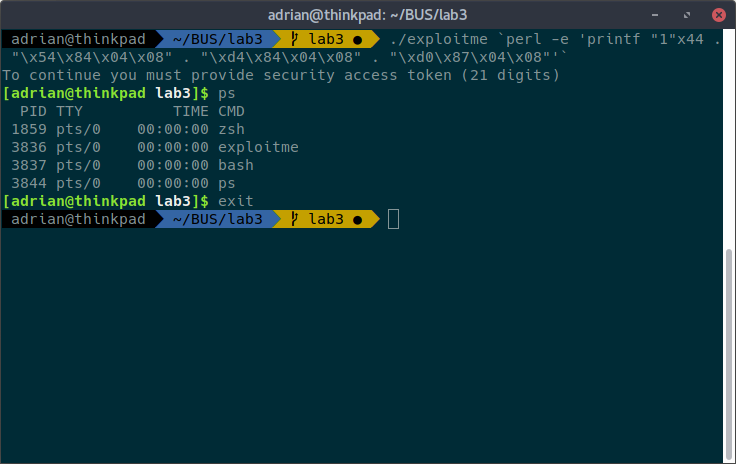
\includegraphics[width=.9\textwidth]{scr.png}
\end{figure}

\end{document}